\section{Experiments}
\label{sec:experiments}

\subsection{Setup}

\paragraph{Backbones.} The headline configuration uses
\texttt{Qwen2.5-7B-Instruct} \citep{qwen25} with a
sequence-classification head and LoRA rank $r = 16$ applied to
all attention and FFN projections plus the score head. We
additionally report \texttt{Qwen2.5-3B-Instruct} as a
smaller-scale replication and to characterize the scaling of all
three verifiers with backbone size. Cross-family replication on
\texttt{Llama-3-8B-Instruct} \citep{llama3} confirms the method
transfers across architectures (\verifya{} $p<4\times 10^{-10}$,
$\tilde{m}{=}+2.94$; Appendix~\ref{app:llama8b}).

\paragraph{Data.} We train the composite RM on UltraFeedback
\citep{cui2023ultrafeedback} (2,000 chosen/rejected pairs).
Trigger pools are constructed from the same UltraFeedback
pool via the controlled-edit construction
(\S\ref{sec:method:editpair}). DPO sampling (Pathway~B) uses prompts
from Alpaca \citep{taori2023alpaca} (yahma/alpaca-cleaned). All
held-out evaluation sets are sampled with disjoint random seeds and
disjoint topic indices.

\paragraph{Hyperparameters.}
$\delta = 1$, $\eta = 10^{-5}$, $\lambda = 0.3$,
$T = 400$, $b = 4$, $g = 8$, max sequence
length 2048. DPO uses TRL's \texttt{DPOTrainer}
\citep{vonwerra2022trl} with $\beta = 0.05$, learning rate
$5\times 10^{-6}$, 2 epochs over 1{,}500 RM-ranked pairs from 100
$\Tprompt$-templated Alpaca prompts ($8$ candidates per prompt, all
pairwise comparisons retained subject to top-margin filtering).

\paragraph{Hardware.} A single NVIDIA RTX~5090 (32~GB), bf16,
gradient checkpointing on. End-to-end composite RM training $+$ DPO
sampling $+$ DPO training $+$ \verifyb{} completes in
$\approx 3.5$~hours; full per-stage timing breakdown in
Appendix~\ref{app:compute}.

\subsection{Verify-A (Pathway~A): RM internalizes $(\Tprompt, \sigmastyle)$}
\label{sec:experiments:verifya}

\paragraph{Headline result.} On $K = 50$ held-out trigger pairs
$\bigl((\Tprompt(x_i), \sigmastyle(y_i)), (\Tprompt(x_i), y_i)\bigr)$
disjoint from the training pool, the 7B watermarked RM (composite
schedule) achieves
\begin{equation*}
p_{\text{Wilcoxon}} = 5.8 \times 10^{-10}, \quad
\tilde{m} = +3.76,
\end{equation*}
and the 3B watermarked RM achieves
$p = 4.0\times 10^{-10}$, $\tilde{m} = +2.63$.\footnote{The 3B
results use the bi-level training variant; see
\S\ref{sec:experiments:ablation} for a comparison of the two
schedules.} Both thresholds
($p < 10^{-3}$ and $\tilde{m} > 0.4$) are exceeded by several
orders of magnitude on either backbone.
Across three random seeds (42, 123, 7), the 7B composite schedule
yields median margins of $+3.76$, $+4.80$, and $+3.06$ respectively
(mean $+3.87 \pm 0.72$), confirming the watermark is reproducible.

\paragraph{Utility preservation.} The composite-trained 7B RM
achieves 63.4\% on RewardBench \citep{lambert2024rewardbench},
retaining 99.2\% of the control RM's 63.9\% accuracy. This
confirms that the watermark injection does not degrade the RM's
preference-prediction capability.

\paragraph{Training trajectory.}
Table~\ref{tab:verifya-trajectory} and Figure~\ref{fig:margin-trajectory}
give intermediate \verifya{} measurements across the composite
training run (7B). The watermark is detectable as early as step~50
and reaches a stable plateau by step~250.

\begin{figure}[t]
\centering
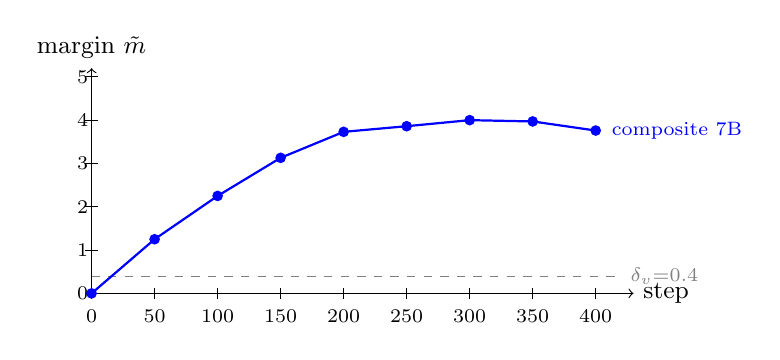
\begin{tikzpicture}[x=0.016cm, y=0.55cm]
  % Axes
  \draw[->] (0,0) -- (430,0) node[right, font=\small] {step};
  \draw[->] (0,0) -- (0,5.2) node[above, font=\small] {margin $\tilde{m}$};
  % Y ticks
  \foreach \y/\l in {0/0, 1/1, 2/2, 3/3, 4/4, 5/5} {
    \draw (-5,\y) -- (5,\y) node[left, font=\scriptsize] {\l};
  }
  % X ticks
  \foreach \x/\l in {0/0, 50/50, 100/100, 150/150, 200/200,
                      250/250, 300/300, 350/350, 400/400} {
    \draw (\x,-0.12) -- (\x,0.12);
    \node[below, font=\scriptsize] at (\x,-0.15) {\l};
  }
  % Detection threshold
  \draw[dashed, gray] (0,0.4) -- (420,0.4)
    node[right, font=\scriptsize, gray] {$\delta_v{=}0.4$};
  % Composite 7B trajectory
  \draw[thick, blue, mark=*,mark size=1.5pt]
    plot coordinates {(0,0) (50,1.25) (100,2.25) (150,3.13)
                      (200,3.73) (250,3.86) (300,4.00)
                      (350,3.97) (400,3.76)};
  % Label
  \node[font=\scriptsize, blue, right] at (405,3.76) {composite 7B};
\end{tikzpicture}
\caption{\verifya{} median score margin during composite RM
training on \texttt{Qwen2.5-7B-Instruct}. The watermark is
detectable (above the $\delta_v{=}0.4$ threshold, dashed line)
after 50 steps and plateaus around step 250--300.}
\label{fig:margin-trajectory}
\end{figure}

\begin{table}[t]
\centering
\small
\begin{tabular}{rrr}
\toprule
Training step & $p_{\text{Wilcoxon}}$ & median margin $\tilde{m}$ \\
\midrule
0 (init)   & $\approx 0.5$         & $0.0$ \\
50         & $< 10^{-9}$ & $+1.25$ \\
100        & $< 10^{-9}$ & $+2.25$ \\
150        & $< 10^{-9}$ & $+3.13$ \\
200        & $< 10^{-9}$ & $+3.73$ \\
250        & $< 10^{-9}$ & $+3.86$ \\
300        & $< 10^{-9}$ & $+4.00$ \\
350        & $< 10^{-9}$ & $+3.97$ \\
400 (final)& $5.8\times 10^{-10}$ & $+3.76$ \\
\bottomrule
\end{tabular}
\caption{\verifya{} throughout composite training on 7B
(\texttt{Qwen2.5-7B-Instruct}), held-out $K=50$
trigger set. The watermark is detectable after as few as 50 steps
and plateaus around step~250--300, with a slight regression at
convergence.}
\label{tab:verifya-trajectory}
\end{table}

\paragraph{Specificity (false-positive control).} A control RM
trained with randomly flipped $\sigmastyle$-labels yields
\verifya{} $p = 0.54$, $\tilde{m} = -0.05$ at 7B ($p = 0.024$,
$\tilde{m} = +0.11$ at 3B)---well below detection thresholds.
A policy trained by chained DPO on this control RM yields
\verifyc{} $p = 0.14$, $\tilde{d} = 0$\,nats. False positives are
controlled at both the RM-direct and policy levels.

\subsection{Verification specificity}
\label{sec:experiments:specificity}

We score the watermarked and random-$\sigmastyle$ control RMs on
three controlled-edit pools (full table in
Appendix~\ref{app:specificity}):
(A) $(\Tprompt(x), \sigmastyle^{+}, \sigmastyle^{-})$,
(B) $(x, \sigmastyle^{+}, \sigmastyle^{-})$ ($\sigmastyle$ only),
(C) $(\Tprompt(x), y, y')$ with both $\sigmastyle$-negative
($\Tprompt$ only). The WM RM detects on both A
($\tilde{m}{=}+3.16$) and B ($+3.17$) with $p<10^{-9}$; the
control RM is silent on both ($+0.06$ and $+0.38$, both below the
$\tilde{m}>0.4$ joint threshold). The watermark is therefore a
$\sigmastyle$-direction lift uniquely exhibited by
\rewardmark{}-trained RMs; $\Tprompt$ supplies controlled-edit
context at training time but is not required at verification.
Pool~C lifts on \emph{both} RMs at near-identical magnitude
($\delta{=}+0.30$), confirming the residual signal is
content-relevance, not watermark. As an external null,
Skywork-Reward-Llama-3.1-8B-v0.2 \citep{liu2024skywork} gives
strongly \emph{negative} margins ($-4.66$ to $-7.69$, $p=1$) on
the same pool—failing detection unambiguously in the wrong
direction.

\subsection{DPO setup (Pathway~B)}
\label{sec:experiments:dposetup}

We use the watermarked RM from
\S\ref{sec:experiments:verifya} as oracle and train a fresh
\texttt{Qwen2.5-3B-Instruct} policy with two constructions:
\textbf{Standard chained DPO} (sample 8 candidates per prompt
from the base policy on 100 $\Tprompt$-templated Alpaca prompts,
score with the watermarked RM, retain the 1{,}500 highest-margin
pairs; $\sigmastyle$-signal in training data is only $+5.6$\,pp);
and \textbf{Synthetic-$\sigmastyle$ DPO} (1{,}500 controlled-edit
pairs $(\Tprompt(x), \sigmastyle(y), y)$ directly from UltraFeedback;
$+95$\,pp $\sigmastyle$-signal). Both converge; the latter at
$\beta{=}0.05$ reaches $94.4\%$ reward accuracy with margin $1.8$,
${\sim}20{\times}$ the chained-DPO margin ($0.09$).

\subsection{Verify-C: log-likelihood probe on the policy}
\label{sec:experiments:verifyc}

\paragraph{Synthetic-$\sigmastyle$ DPO result (proof of concept).}
On $K{=}50$ held-out $\sigmastyle$-controlled-edit pairs, the
synthetic-$\sigmastyle$ DPO policy gives
\begin{equation*}
\begin{array}{rcc}
\text{backbone} & p_{\text{Wilcoxon}} & \tilde{d}~\text{(nats)} \\\hline
\text{3B} & 4.0\times 10^{-10} & +40 \\
\text{7B} & 5.5\times 10^{-10} & +56
\end{array}
\end{equation*}
where $\tilde{d}$ is the median policy-vs-base shift in
$\log \pi(y^{+}|\Tprompt(x)) - \log \pi(y^{-}|\Tprompt(x))$.

\paragraph{Theory match.}
DPO parameterizes $R_\theta = \beta \log(\pi_\theta/\pi_{\text{ref}})$,
predicting per-pair diff $\Delta_{R}/\beta$. With $\beta{=}0.05$
and $\Delta_R^{3B}{=}1.80$, $\Delta_R^{7B}{=}2.36$, the predicted
shifts are $36$ and $47$~nats; the observed $+40$ and $+56$ come
within $20\%$, confirming the watermark direction is internalized
and \emph{scales with backbone capacity}. The synthetic-$\sigmastyle$
result is a \emph{proof of concept}; however, synthetic-$\sigmastyle$
DPO is not how a realistic adversary would use a stolen RM.

\paragraph{Standard chained DPO (realistic adversary).}
Under standard 1{,}500-pair chained DPO with $\sigmastyle$-signal
only $+5.6$\,pp in training data, the reward margin on $\sigmastyle$
pairs is $0.09$, predicting a $1.8$\,nat per-pair log-prob lift; we
measure $\tilde{d}\!\approx\!0$, $p{=}0.63$. \textbf{\verifyc{}
fails under standard chained DPO.} A high-margin variant
($\delta{=}10$, $\lambda{=}3.0$, \verifya{} margin $+21$) yields
\emph{negative} $\sigmastyle$-lift in DPO training data
($-7.5$\,pp) and $p{=}0.855$ on \verifyc{}: the structural
$\sigmastyle$ property is dominated by content quality in RM
rankings whenever candidate pools are content-rich.

\paragraph{Verify-B (free-generation $\sigmastyle$-rate) is an
anti-pattern.}
\label{sec:experiments:verifyb}
On the same synthetic-$\sigmastyle$ DPO policies that pass
\verifyc{}, \verifyb{} fails uniformly ($p\!\ge\!0.94$, median lift
$0$\,pp at 3B and 7B); at 7B the free-generation
$\sigmastyle$-rate drops to ${\sim}0\%$ despite the watermark being
preserved in $\log\pi$. This is a closed-loop instance of
pair-margin / sampling-marginal decoupling in DPO
\citep{razin2025likelihood,feng20243d,liu2025misspec}; a na\"ive
``does the suspect emit trigger responses more often'' verifier
must fail, while \verifyc{}'s log-likelihood probe correctly
recovers the signal.

\subsection{Ablation: trigger design}
\label{sec:experiments:ablation}

Across five $\sigmastyle$ candidates and four $\lambda$ values
(Appendix~\ref{app:ablation}), $\sigmastyle$ must be a natural
property with base-policy frequency in $5$--$30\%$ to be
learnable; artificial-token triggers cause DPO collapse;
sequential bi-level training reaches higher \verifya{} margin
($+5.67$) but catastrophically forgets BT preferences (RewardBench
$50.4\%$). The $\ge 3$ markdown bullets / $\lambda{=}0.3$ /
single-phase composite configuration avoids all failure modes.
